%!TEX root = ../template.tex
%%%%%%%%%%%%%%%%%%%%%%%%%%%%%%%%%%%%%%%%%%%%%%%%%%%%%%%%%%%%%%%%%%%%
%% chapter4.tex
%% NOVA thesis document file
%%
%% Chapter with lots of dummy text
%%%%%%%%%%%%%%%%%%%%%%%%%%%%%%%%%%%%%%%%%%%%%%%%%%%%%%%%%%%%%%%%%%%%

\typeout{NT FILE chapter4.tex}%

\chapter{RPC}
\label{cha:RPC}

%\epigraph{
%	"What we observe is not nature itself, but nature exposed to our method of questioning."
%}{Werner Heisenberg}
\epigraph{
	"The scientist is not a person who gives the right answers, but one who asks the right questions — and builds the tools to answer them."
}{Claude Lévi-Strauss (paraphrased)}
%\epigraph{
%	"Precision is not just about measurement — it is about insight."
%}



\section{Introduction and Historical Context}

Resistive Plate Chambers (RPCs) are gaseous ionization detectors introduced in the early 1980s as a cost-effective solution for large-area charged-particle detection with excellent time resolution. Their working principle relies on the formation of localized electron avalanches in a thin gas gap between two resistive electrodes, typically made of glass or bakelite, under a strong uniform electric field \cite{riegler_physics_2004}. When a charged particle traverses the gas volume, it ionizes the medium, creating primary electron-ion pairs. The applied electric field accelerates the liberated electrons, initiating an avalanche multiplication process that induces a fast signal on metallic readout strips placed outside the resistive electrodes.

The original single-gap RPC design offered sub-nanosecond timing capabilities and good detection efficiency at relatively low cost, making it widely adopted in high-energy physics experiments. Subsequent developments led to the introduction of Multi-Gap Resistive Plate Chambers (MRPCs), which consist of several narrow gas gaps arranged in parallel between resistive plates \cite{riegler_physics_2004}. This configuration enhances the detector’s timing precision by reducing statistical fluctuations in avalanche development and limiting the overall charge per avalanche, improving rate capability and stability. MRPCs have become the standard in modern time-of-flight (TOF) systems in nuclear and particle physics, delivering intrinsic time resolutions below 50 ps for minimum ionizing particles (MIPs) and efficiencies exceeding 98\% \cite{blanco_ship_2020}.

Due to their scalability, robustness, and excellent timing performance, RPCs and MRPCs are extensively employed in experiments at facilities such as CERN, GSI, and RHIC, particularly in large TOF walls and tracking systems. Their application in relativistic heavy-ion collisions, rare-isotope beam experiments, and cosmic-ray detectors demonstrates their versatility and importance in modern experimental physics.

\section{Detector Design, Construction, and Properties}

The Resistive Plate Chamber (\gls{RPC}) implemented in the \gls{R3B} experimental setup at GSI is a large-area timing detector developed for precise identification of charged fragments in relativistic heavy-ion collisions \cite{blanco_ship_2020}. It is based on the Multi-Gap RPC (MRPC) concept, which significantly enhances timing performance through multiple narrow gas gaps that ensure stable avalanche development.

The detector comprises two identical modules, each hosting a six-gap glass stack, giving a total of twelve 0.3 mm-thick gas gaps per detection plane. These gaps are defined by fishing lines to guarantee uniform separation between the electrodes. The electrodes themselves consist of 1 mm-thick float glass coated with a resistive layer that provides uniform high-voltage distribution. Together, the modules form an active detection area of 1550 × 1250 mm$^2$ (1.94 m$^2$), making this RPC one of the largest deployed in nuclear physics experiments.

The readout system is composed of 41 copper strips, each 29 mm wide and 1600 mm long, arranged on a central PCB placed between the two modules. Each strip is read out on both ends, referred to as the left and right sides. This configuration enables reconstruction of the Y-position from the strip index and the X-position from the signal arrival time difference between both ends. Timing measurements are performed using front-end electronics based on NINO ASICs, which provide fast leading-edge discrimination and time-over-threshold (ToT) encoding. The digitization stage employs TRB boards equipped with multi-channel TDCs featuring sub-30 ps resolution, ensuring precise timing measurements even under high-rate conditions.

The detector operates in avalanche mode with a gas mixture of 98\% tetrafluoroethane (C$_2$H$_2$F$_4$) and 2\% sulfur hexafluoride (SF$_6$), maintained slightly below atmospheric pressure. The working voltage is approximately 3 kV per gap, resulting in a total applied potential of $\sim$18 kV per module. This configuration ensures efficient avalanche formation while suppressing streamer transitions and electrical breakdown.

Performance benchmarks obtained in previous tests and beam time campaigns confirm the excellent capabilities of this RPC design. The detector achieves a timing resolution of 50–80 ps for minimum ionizing particles in controlled conditions, and approximately 80–100 ps in realistic beam environments, where additional contributions from reference detectors and beam spread are included. The detection efficiency exceeds 95\% under beam conditions and can reach 98\% in optimized laboratory setups. Spatial resolution is governed by the 29 mm strip pitch in the vertical direction and the signal propagation velocity along the strip for the horizontal position, yielding sub-centimeter accuracy in X after calibration \cite{blanco_ship_2020, xarepe_resistive_2023}.

A schematic representation of the detector geometry and strip layout is shown in Figure \ref{fig:RPCScheme}.

\begin{figure}[H]
	\centering
	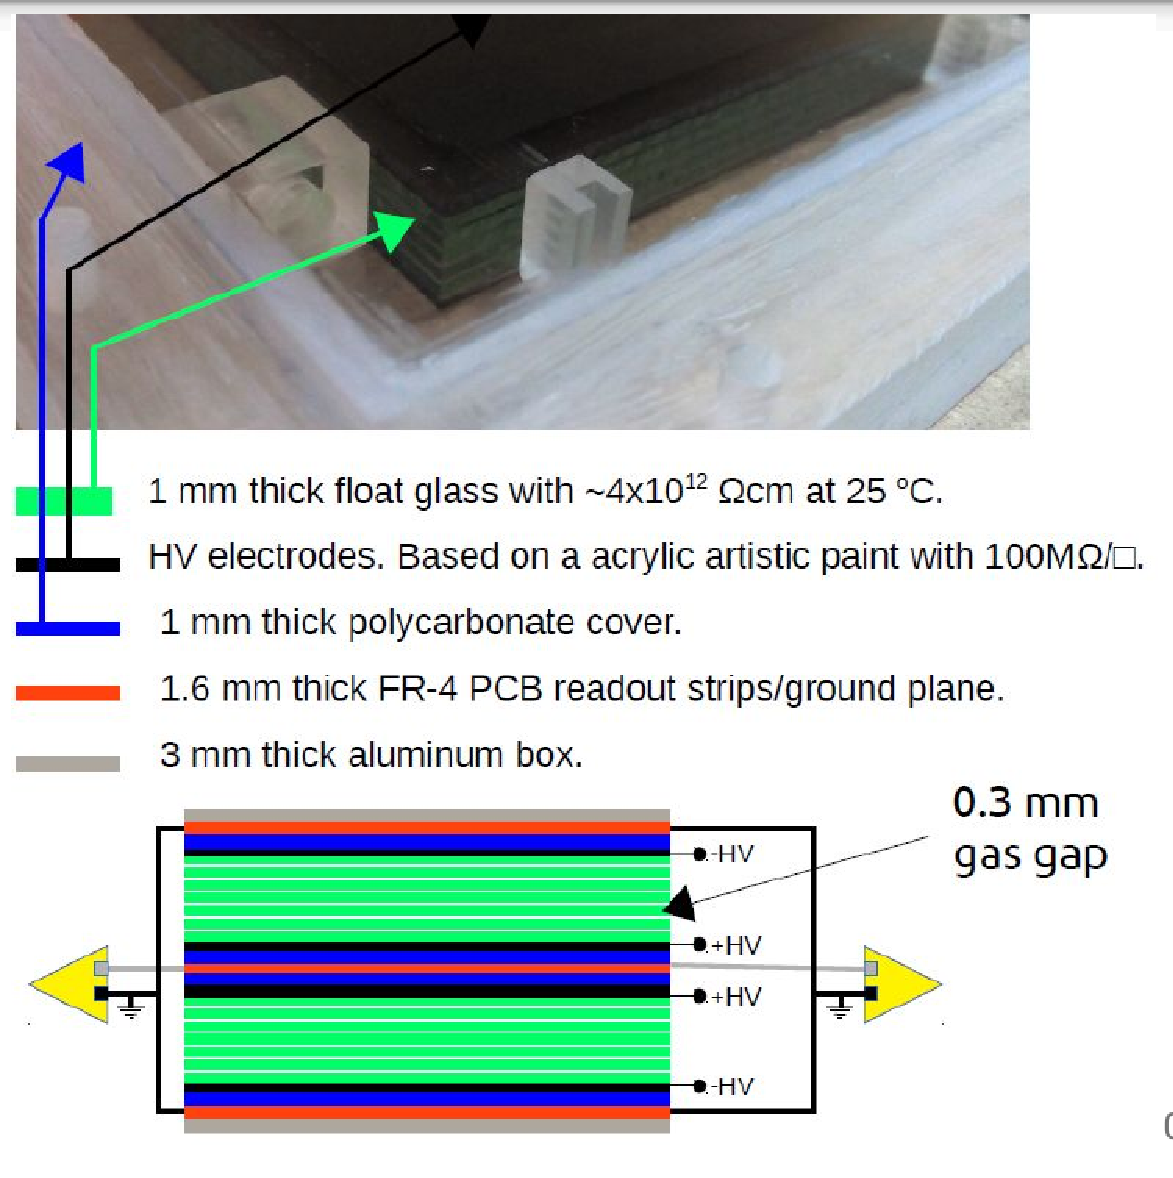
\includegraphics[width=\linewidth]{RPC Schematic}
	\caption{Schematic representation of the top view of the RPC. Reprinted from \cite{blanco_ship_2020}.}
	\label{fig:RPCScheme}
\end{figure}
      


\section{Operating Principle and Gas System}

\subsection{Gas Mixture and Physics Motivation}

The \gls{RPC} operates with a carefully selected gas mixture composed of 98\% tetrafluoroethane (C$_2$H$_2$F$_4$), also known as R-134a or Freon, and 2\% sulfur hexafluoride (SF$_6$). This specific combination plays a critical role in establishing a stable and efficient ionization environment, ensuring optimal charge amplification and suppression of undesired discharges.
\\
\\
\textbf{C$_2$H$_2$F$_4$ (Tetrafluoroethane)}

As the primary component of the mixture, C$_2$H$_2$F$_4$ serves as the ionization medium and is responsible for supporting electron avalanches. Charged particles traversing the detector ionize the gas, liberating electrons that are accelerated by the applied electric field. Due to its moderate ionization energy ($\sim$13.10 eV) \cite{pereira-da-silva_electron_2021}, C$_2$H$_2$F$_4$ enables efficient impact ionization, resulting in the formation of localized electron avalanches. Its polyatomic molecular structure provides internal vibrational modes that help absorb excess energy, thus preventing the transition to streamer mode. Furthermore, its relatively low electron diffusivity promotes spatially confined signal generation, preserving time resolution and detector stability.
\\
\\
\textbf{SF$_6$ (Sulfur Hexafluoride)}

Although present in a small fraction, {SF$_6$ is vital to the safe operation of the \gls{RPC}. As a strongly electronegative gas, {SF$_6$ captures free electrons and suppresses excessive avalanche growth, thus preventing transitions to streamer or breakdown regimes. It also serves as a quenching agent by absorbing ultraviolet photons emitted by excited C$_2$H$_2$F$_4$ molecules, which would otherwise induce secondary avalanches. Through these mechanisms, {SF$_6$ enhances the stability of the avalanche mode and significantly improves timing performance.

\subsection{Operating Pressure}

The internal pressure of the \gls{RPC} is maintained slightly below atmospheric levels. This configuration is mechanically advantageous, as the higher external atmospheric pressure effectively compresses the detector structure, keeping the glass stacks firmly aligned and minimizing the risk of internal gaps or misalignments.

\subsection{Detector Operating Modes}

The \gls{RPC} can, in principle, operate in three distinct regimes:

\begin{itemize}
	\item Avalanche Mode (Preferred): The detector operates with controlled charge multiplication, producing fast, localized signals with minimal dead time. The presence of SF$_6$ is crucial to maintaining operation in this regime.
	\item Streamer Mode (Undesired): Inadequate quenching may lead to excessive avalanche growth and transition to streamer discharges, degrading time and spatial resolution and risking damage to the detector.
	\item Breakdown Mode (Failure): In the absence of sufficient suppression mechanisms, an uncontrolled discharge may occur, leading to continuous current flow and permanent damage to the detector plates.
\end{itemize}

The selected gas mixture and voltage operating point are tuned specifically to maintain operation within the avalanche mode, maximizing performance and longevity.


\section{Readout Electronics and Signal Reconstruction}

The \gls{RPC} detector is read out using a differential system in which each of the signal strips is instrumented on both ends—referred to as the left and right sides. For each event in which a signal crosses a predefined threshold, the readout system records the strip number, the leading and trailing edge times (i.e., the time when the signal crosses the threshold on both the rising and falling edges), and the side (left or right) on which the signal was detected.

From this raw information, a hit can be reconstructed by extracting three key physical quantities: the spatial coordinates of the hit on the detector plane (X and Y), and the time information necessary for further analysis and event building.

\begin{itemize}
	\item Y-position: The vertical position of the hit is determined directly from the strip number. Each strip has a fixed pitch (in this case, 3 cm), so the position along the Y-axis is given by the centerline of the corresponding strip.
	\item X-position: The horizontal position along the strip is reconstructed using the time difference between the left and right sides. Assuming a known signal propagation speed along the strip, the hit position is computed from the time asymmetry:
	\[X = \frac{1}{2}(t_{right} - t_{left})\]
	where $t_{right}$ and $t_{left}$​ are the leading edge times on each end. This method assumes uniform propagation speed and symmetric signal shape, which are validated through calibration.
	\item Time Over Threshold (ToT): The time over threshold is defined as the difference between the trailing and leading edge times for a given signal. It provides an estimate of the pulse height (i.e., deposited charge) and is used as a quality criterion to discriminate valid hits from noise. Only signals with a ToT value within an expected range are accepted for further reconstruction.
\end{itemize}

This digital processing chain—from raw timing and strip information to physically meaningful hit coordinates—is integrated into the \gls{R3B} data processing framework. It enables high-resolution tracking and time measurement, critical for associating \gls{RPC} hits with particle trajectories and for synchronization with the rest of the \gls{R3B} detector systems.

\section{Performance in Previous Beam Time}

The \gls{RPC} system underwent its first test during beam time at the \gls{R3B} setup and demonstrated excellent performance \cite{xarepe_resistive_2023}. The detector achieved an efficiency exceeding 95\%, with reliable synchronization with the rest of the \gls{R3B} detectors. The data acquisition was stable over the full two-week operation period, confirming the robustness of both the hardware and software components.

\begin{figure}[H]
	\centering
	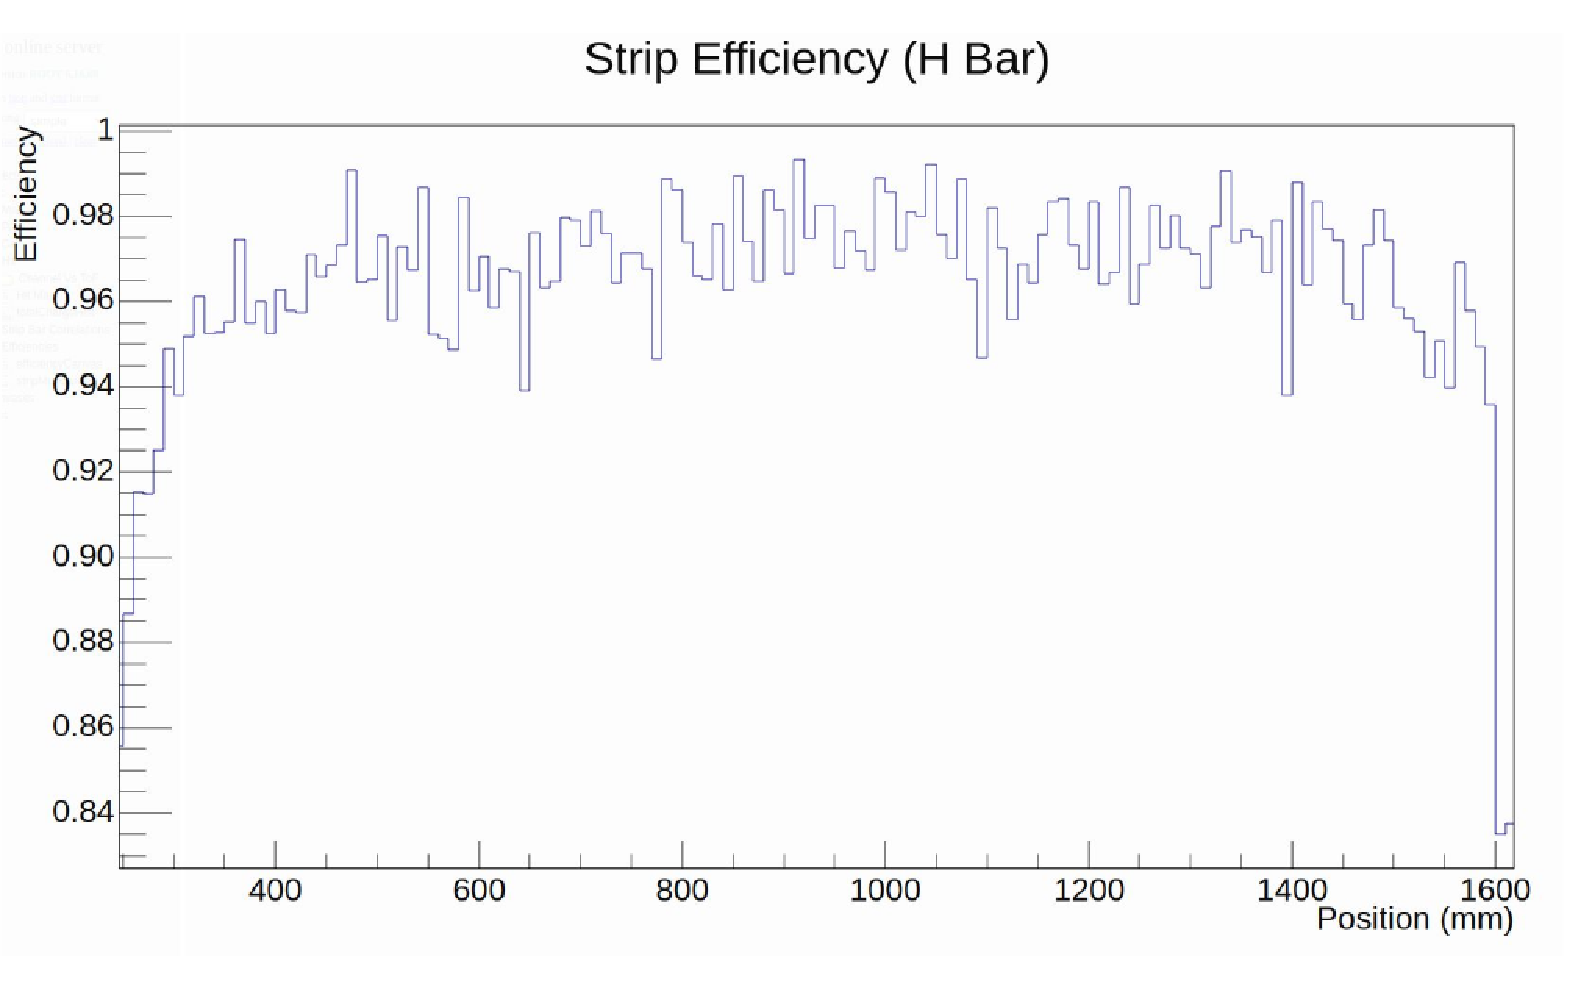
\includegraphics[width=0.8\linewidth]{RPC Strip Efficiency}
	\caption{Measured strip efficiency of the RPC during beam time.}
	\label{fig:RPCStripEff}
\end{figure}

\section{Role of the RPC in the Present Experiment}

In previous implementations within the \gls{R3B} experimental setup, the \gls{RPC} was primarily employed for the detection and timing of protons, operating under well-controlled conditions with relatively low particle multiplicity. The present experiment introduces a new challenge for the detector: the need to process a broader variety of charged particles, including heavier fragments. This scenario represents an important step in validating the \gls{RPC} technology for more complex experimental conditions, aligning with future applications in \gls{FAIR} and NUSTAR.

The motivation behind testing the \gls{RPC} under these conditions lies in assessing its efficiency, timing performance, and overall stability when exposed to an extended particle spectrum beyond protons. Such an evaluation is critical for determining the feasibility of using \gls{RPC}s as precision timing detectors in high-intensity, high-multiplicity environments, particularly where versatility in particle identification is required.


\section{Detector Preparation Procedure}

The preparation of the \gls{RPC} prior to beam time involves several carefully controlled steps to ensure proper gas composition, structural stability, and operational calibration:

\begin{enumerate}
	\item Drying Phase: Before filling with the working gas mixture, the \gls{RPC} is flushed for several days with SF$_6$ to remove residual moisture. As a more cost-effective alternative, nitrogen was used for this purpose; however, care must be taken to avoid over-pressurization, which could damage the delicate glass structure.
	\item Leak Testing: Prior to introducing the working gas mixture, the system is tested for leaks. This is done by filling the gas lines while keeping the mass flow controllers closed and monitoring for pressure drops after closing the gas bottles. During this phase, a minor leak was detected. To localize it, various segments of the gas line were isolated and tested independently. These checks did not reveal any leakage in the external tubing, suggesting that the source of the leak was likely located within the \gls{RPC} chamber itself, or at one of the gas inlet or outlet ports. Despite this issue, the leak was sufficiently small that it did not affect the detector’s performance during beam time and did not require immediate intervention.
	\item Gas Insertion and Calibration: Once leak tightness is confirmed, the 98\% C$_2$H$_2$F$_4$ / 2\% SF$_6$ gas mixture is introduced. To determine the optimal operating voltage, the detector is calibrated using cosmic ray coincidence measurements. For this purpose, a vertical NeuLAND bar is placed on each side of the \gls{RPC}. Coincidences allow for the fine adjustment of the high voltage supply to identify the working point that maximizes timing resolution and detection efficiency. An example of these calibration results is presented in Figure \ref{fig:RPC_WorkingPoint}, which illustrates the dependence of efficiency and signal characteristics on the applied high voltage.
\end{enumerate}



The entire preparation process takes approximately two weeks, after which the detector is ready for integration into the experimental campaign.

\begin{figure}[H]
	\centering
	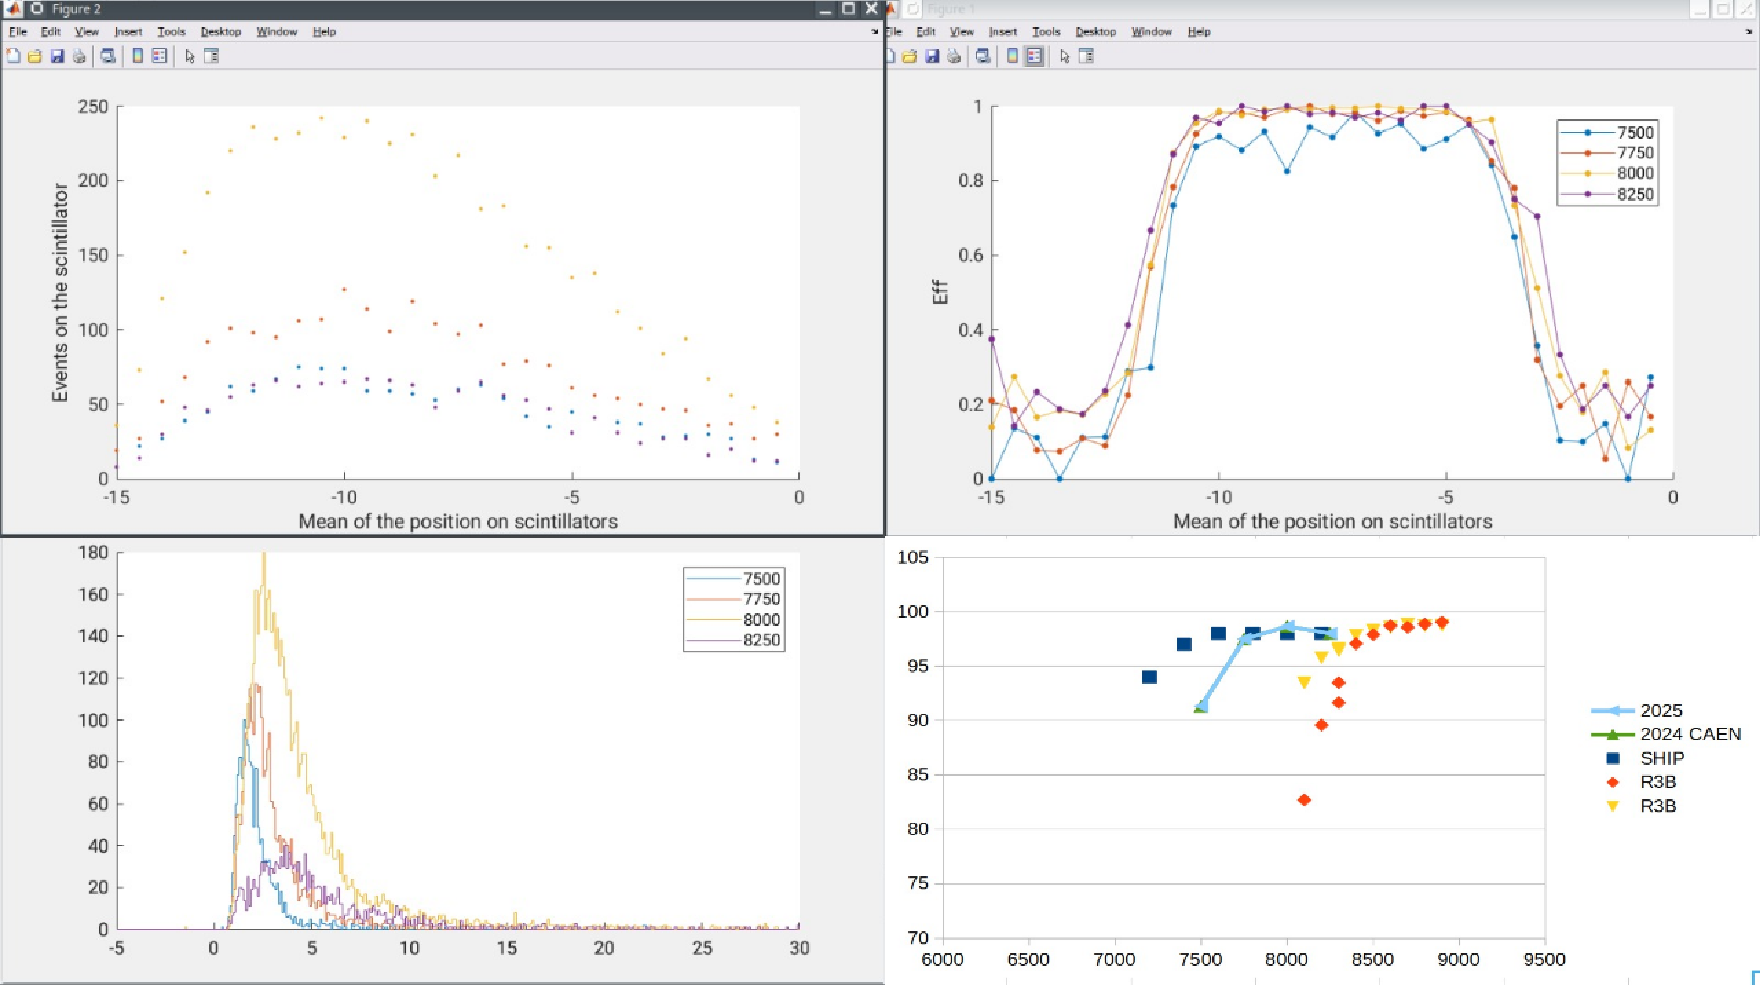
\includegraphics[width=\linewidth]{RPC_WorkingPointCalibration}
	\caption{Calibration of the RPC working point using cosmic ray data. The top-left panel shows the distribution of events as a function of the mean position on the scintillators for different applied voltages. The top-right panel presents the corresponding efficiency curves as a function of position for four high-voltage settings (7500, 7750, 8000, and 8250 V). The bottom-left panel shows the time-over-threshold (ToT) distributions for the same voltages, which are used as a quality criterion for hit selection. The bottom-right panel summarizes the overall efficiency as a function of the applied voltage, including results from previous beam campaigns for comparison.}
	\label{fig:RPC_WorkingPointCalibration}
\end{figure}

\section{Contributions to Detector Operation and Monitoring}

As part of the preparatory and operational phases of the experiment, several tasks related to the control and monitoring of the \gls{RPC} system were developed or improved. These contributions focused on increasing system reliability, enabling remote intervention, and enhancing real-time observability during beam time.

\subsection{Monitoring Infrastructure for RPC Voltage and Current}

To ensure the stable and safe operation of the \gls{RPC}, a custom monitoring script was developed to continuously track the voltage and current supplied to the detector’s resistive plates. This script interfaces with the high-voltage power supply and records the measured parameters at regular intervals. The collected data are automatically transmitted to a Grafana-based visualization dashboard, providing real-time insights into the detector’s electrical behavior. This tool proved essential for diagnosing fluctuations, identifying abnormal conditions during beam time, and maintaining long-term performance stability.
These monitoring plots, generated during beam time, are shown in Figure \ref{fig:RPCGrafana}, where the stability of the applied voltage and the corresponding current drawn by the resistive plates can be visualized over time.

\begin{figure}[H]
	\centering
	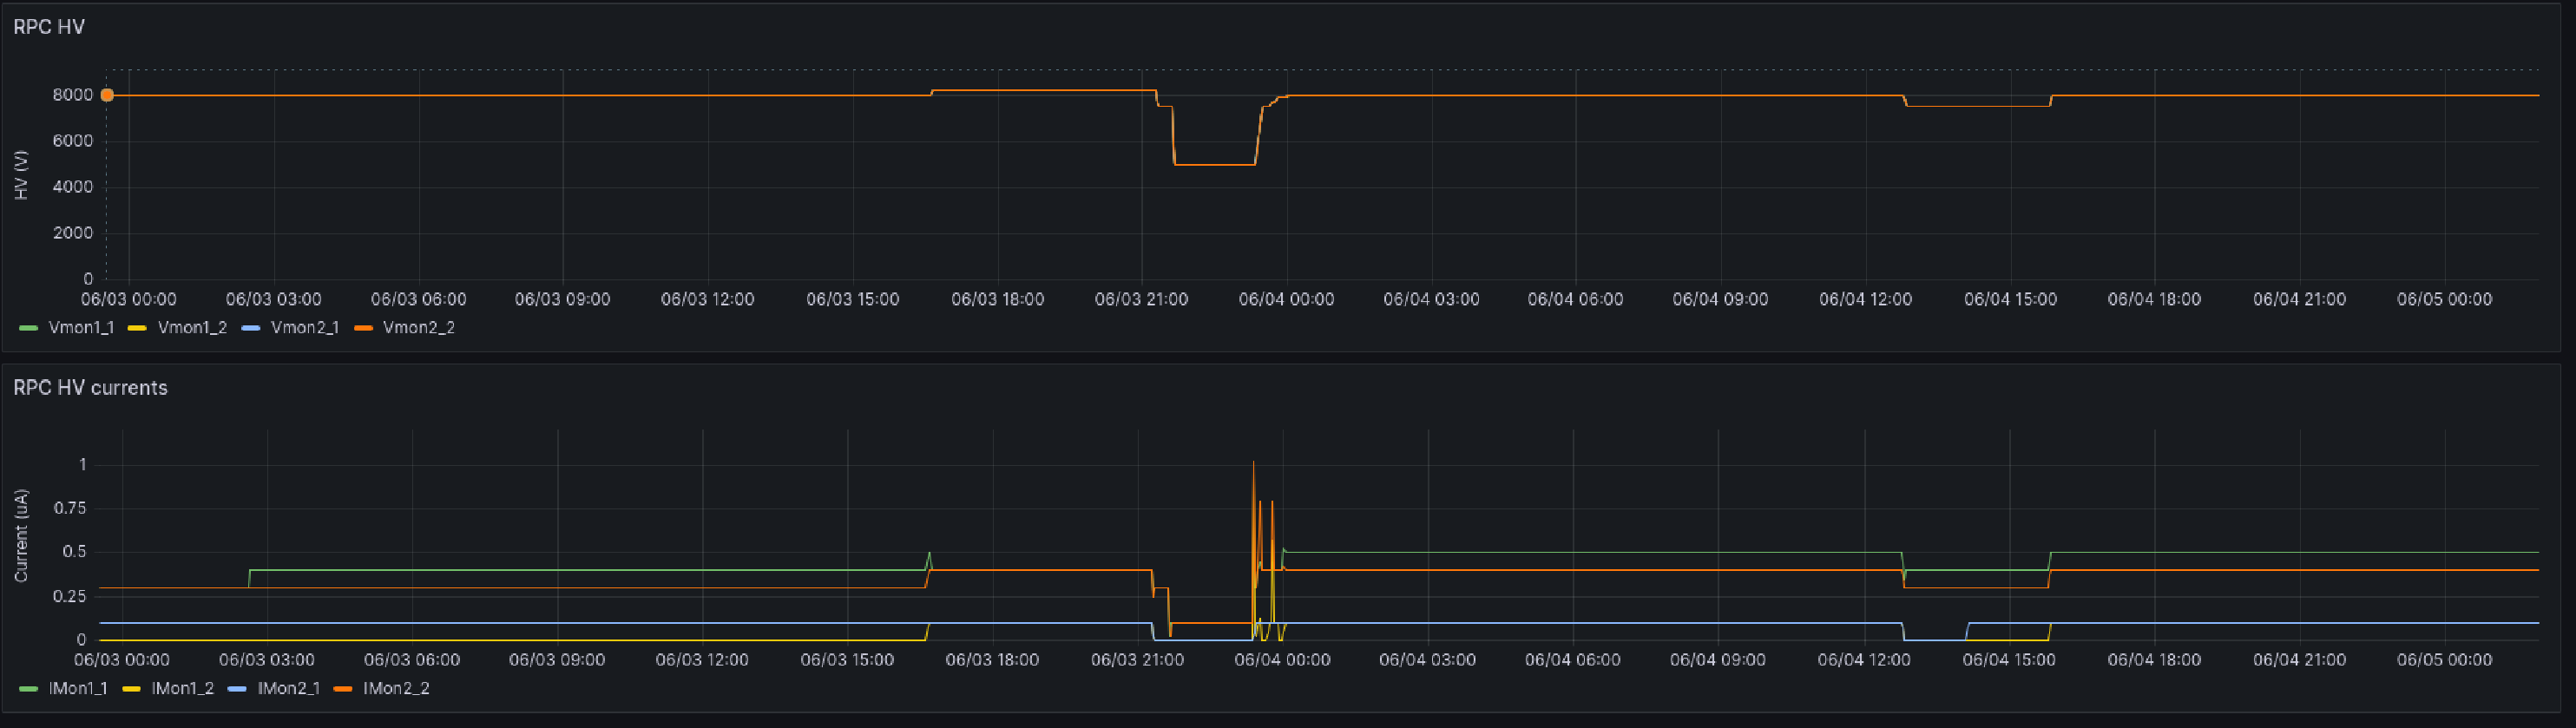
\includegraphics[width=\linewidth]{RPCGrafana}
	\caption{Example of live Grafana dashboard showing voltage and current monitoring of the RPC during beam operation.}
	\label{fig:RPCGrafana}
\end{figure}

\subsection{Remote Control and Recovery Tools}

In addition to monitoring, improvements were made to the \gls{RPC} control interface by updating and correcting a script used for remote power cycling of the detector. This script also allows for the automated restart of the DAQ and acquisition systems, facilitating rapid recovery in the event of software or hardware issues. These functionalities were used during beam time to reinitialize the \gls{RPC} without requiring direct physical access to the electronics rack, minimizing downtime and ensuring uninterrupted data collection.

These tools contributed directly to the detector’s robust operation and were successfully integrated into the experimental workflow.
